\documentclass[uplatex]{jsarticle}
\usepackage[utf8]{inputenc}
% 図を現在位置に挿入
\usepackage{here}
% 文字コード関連の設定
\usepackage{otf}
% 数式
\usepackage{amsmath,amssymb}
\usepackage{empheq}
\usepackage{amsthm}
\newtheorem{dfn}{定義}
\newtheorem{thm}{定理}
\newtheorem{prf}{証明}
\newtheorem{law}{法則}
\newtheorem{ex}{例}
\newtheorem{lemm}{補題}
% 斜体を解除
\makeatletter
\def\th@plain{\upshape}
\makeatother
% フォントエラーを無理やり消す
\DeclareFontShape{JY2}{hmc}{m}{it}{<->ssub*hmc/m/n}{}
\DeclareFontShape{JY2}{hmc}{m}{sl}{<->ssub*hmc/m/n}{}
\DeclareFontShape{JY2}{hmc}{m}{sc}{<->ssub*hmc/m/n}{}
\DeclareFontShape{JT2}{hmc}{m}{it}{<->ssub*hmc/m/n}{}
\DeclareFontShape{JT2}{hmc}{m}{sl}{<->ssub*hmc/m/n}{}
\DeclareFontShape{JT2}{hmc}{m}{sc}{<->ssub*hmc/m/n}{}
\DeclareFontShape{JY2}{hmc}{b}{n}{<->ssub*hmc/bx/n}{}
\DeclareFontShape{JT2}{hmc}{b}{n}{<->ssub*hmc/m/n}{}
% 箇条書きのパラメータ関連の設定
\usepackage{paralist}
% ソースコード関連の設定
\usepackage{listings,jlisting}
% プログラムのソースコード
\lstdefinestyle{program}{
    basicstyle={\small\ttfamily},
    breaklines=true,
    columns=fixed,
    basewidth=0.5em,
    % スペースを可視化するかどうか
    showstringspaces=false,
    % 枠線 trbl(大文字で二重線)
    frame={tb},
    % フレームと本文の間のマージン
    framesep=8pt,
    % 行番号
    numbers=left,
    numbersep=2zw,
    % フォントサイズ
    numberstyle={\scriptsize},
    % マージン
    xrightmargin=0zw,
    xleftmargin=3zw,
    % 行間
    lineskip=-0.2ex,
    % タブ数
    tabsize=4,
    % キャプション名の場所
    captionpos=t,
}
% プログラムの一部
\lstdefinestyle{code}{
    basicstyle={\small\ttfamily},
    breaklines=true,
    columns=fixed,
    basewidth=0.5em,
    % スペースを可視化するかどうか
    showstringspaces=false,
    % フレームと本文の間のマージン
    framesep=8pt,
    % マージン
    xrightmargin=0zw,
    xleftmargin=2.5zw,
    % 行間
    lineskip=-0.2ex,
    % タブ数
    tabsize=4,
}
% コマンド
% 角が丸いフレーム付き(文字サイズsmall)
\lstdefinestyle{command}{
    basicstyle={\small\ttfamily},
    breaklines=true,
    columns=fixed,
    basewidth=0.5em,
    showstringspaces=false,
    frame={trbl},
    frameround={tttt},
    framesep=8pt,
    framerule=0pt,
    xrightmargin=1zw,
    xleftmargin=1zw,
    lineskip=-0.2ex,
    tabsize=4,
}
% 角が丸いフレーム付き
\lstdefinestyle{withframe}{
    basicstyle={\ttfamily},
    breaklines=true,
    columns=fixed,
    basewidth=0.5em,
    showstringspaces=false,
    frame={trbl},
    frameround={tttt},
    framesep=8pt,
    framerule=0pt,
    xrightmargin=1zw,
    xleftmargin=1zw,
    lineskip=-0.5ex,
    tabsize=4,
}
% キャプション名
\renewcommand{\lstlistingname}{プログラム}
% 囲い関連の設定
\usepackage{ascmac}
% マージンの設定
\usepackage[left=30mm,right=30mm,top=30mm,bottom=30mm]{geometry}
\renewcommand{\baselinestretch}{1.15}
% 画像関連
\usepackage[dvipdfmx]{graphicx}
% フォント
\usepackage{newtxtext,newtxmath}
% URL
\usepackage{url}
% 目次
\usepackage[dvipdfmx]{hyperref}
\usepackage{pxjahyper}
\hypersetup{
    setpagesize=false,
    bookmarksnumbered=true,
    bookmarksopen=true,
    colorlinks=true,
    linkcolor=black,
    citecolor=black,
    urlcolor=black
}
% マクロ
% スペース関連
\newcommand{\vsc}{\vspace{5pt}}
\newcommand{\vsp}{\vspace{10pt}}
% コンビネーション
\newcommand{\combination}[2]{{}_{#1} \mathrm{C}_{#2}}
% 順列
\newcommand{\permutation}[2]{{}_{#1} \mathrm{P}_{#2}}
% 重複組み合わせ
\newcommand{\rcombination}[2]{{}_{#1} \mathrm{H}_{#2}}
% ゴシック体のインデントなし
\newcommand{\minisection}[1]{\noindent \textsf{#1}}
% 箇条書きもどき
\newcommand{\likeitem}[1]{
    \noindent
    ○ \, {#1}
}

\begin{document}
\title{タイトル}
\author{名前}
\date{\today}
\maketitle
% 目次生成
\tableofcontents

\newpage
\section{本文}
\subsection{listings}
プログラムは\verb|program|で貼り付ける.

\begin{lstlisting}[style=program,caption=hello.c]
#include <stdio.h>

int main(){
    printf("Hello, World!\n");
    return 0;
}
\end{lstlisting}
\vsp

プログラムの一部は\verb|code|で貼り付ける.

\vsc
\begin{lstlisting}[style=code]
printf("Hello, World!\n");
\end{lstlisting}

コマンドは\verb|command|で貼り付ける.

\vsc
\begin{lstlisting}[style=command]
$ gcc hello.c -o hello
\end{lstlisting}

実行結果などを含む場合も同様.

\vsc
\begin{lstlisting}[style=command]
$ echo "hello"
hello
\end{lstlisting}

単純に囲みたい場合は\verb|withframe|で貼り付ける.

\vsc
\begin{lstlisting}[style=withframe]
TEST    START
        LAD     GR0,15
        LAD     GR1,6
        CALL    DIV
        CALL    OUTDEC
        LD      GR0,GR1
        CALL    OUTDEC
        RET
        END
\end{lstlisting}

\newpage
\subsection{数式}
本文中に数式を入れる場合は\,\verb|$|\,で囲む
(例.$y=ax+b$).

番号付き数式は\,\verb|equation|,番号なし数式は\,\verb|equation*|\,を使う.
\begin{equation}
    \zeta (z) = \sum_{n=1}^{\infty}\frac{1}{n^2}
\end{equation}
\begin{equation*}
    \zeta (z) = \sum_{n=1}^{\infty}\frac{1}{n^2}
\end{equation*}

複数行の数式は\,\verb|align|\,を使う.
\begin{align}
    I   &=  \int_{0}^{1} 3x^2 \,dx \\
        &=  1
\end{align}

連立方程式は\,\verb|empheq|\,を使う
\footnote{\url{https://muscle-keisuke.hatenablog.com/entry/2015/11/23/122725}}.
\begin{empheq}[left=\empheqlbrace]{align}
    a_1x_1 + b_1y_1 + c_1z_1 &= 1\\
    a_2x_2 + b_2y_2 + c_2z_2 &= 2\\
    a_3x_3 + b_3y_3 + c_3z_3 &= 3
\end{empheq}
\begin{empheq}[left={|x|=\empheqlbrace}]{alignat=2}
    x & \quad (x\geq0) \\
    -x & \quad (otherwise)
\end{empheq}

\verb|\displaystyle|\,なし:
$p_n(x) =\sum_{i=0}^n f[x_0,\cdots,x_i] \prod_{j=0}^{i-1}(x-x_j)$

\verb|\displaystyle|\,あり:
$\displaystyle p_n(x) =\sum_{i=0}^n f[x_0,\cdots,x_i] \prod_{j=0}^{i-1}(x-x_j)$

括弧のサイズを合わせる.
\begin{equation}
    (\frac{1}{n})
\end{equation}
\begin{equation}
    \left(\frac{1}{n}\right)
\end{equation}

\begin{itemize}
    \item \verb|matrix|
    \begin{equation}
    \begin{matrix}
        a & b \\
        c & d 
    \end{matrix}
    \end{equation}
    \item \verb|pmatrix|
    \begin{equation}
    \begin{pmatrix}
        a & b \\
        c & d 
    \end{pmatrix}
    \end{equation}
    \item \verb|bmatrix|
    \begin{equation}
    \begin{bmatrix}
        a & b \\
        c & d 
    \end{bmatrix}
    \end{equation}
    \item \verb|vmatrix|
    \begin{equation}
    \begin{vmatrix}
        a & b \\
        c & d 
    \end{vmatrix}
    \end{equation}
    \item \verb|Vmatrix|
    \begin{equation}
    \begin{Vmatrix}
        a & b \\
        c & d 
    \end{Vmatrix}
    \end{equation}
\end{itemize}

\begin{screen}
    \begin{thm}(フェルマーの小定理)\\
        \label{fermat}
        $p$ が素数で $x \in \mathbb{Z}$ が $p$ で割り切れなければ,
        $x^{p-1} \equiv 1 \mod{p}$.
    \end{thm}
\end{screen}

\begin{prf}
    (定理\ref{fermat}の証明)

    頑張ってね.
\end{prf}

\begin{ex}
    こんな感じで例を書く.
\end{ex}

\subsection{マクロによる数式}
\likeitem{順列}

\begin{equation}
    \permutation{n}{r} = \frac{n!}{(n-r)!}
\end{equation}

\likeitem{組み合わせ}

\begin{equation}
    \combination{n}{r} = \frac{n!}{r!(n-r)!}
\end{equation}

\likeitem{重複組み合わせ}

\begin{equation}
    \rcombination{n}{r} = \frac{(n+r-1)!}{r!(n-1)!}
\end{equation}


\newpage
\subsection{図}
\begin{itemize}
    \item 画像の場合
    \begin{figure}[H]
        \centering
        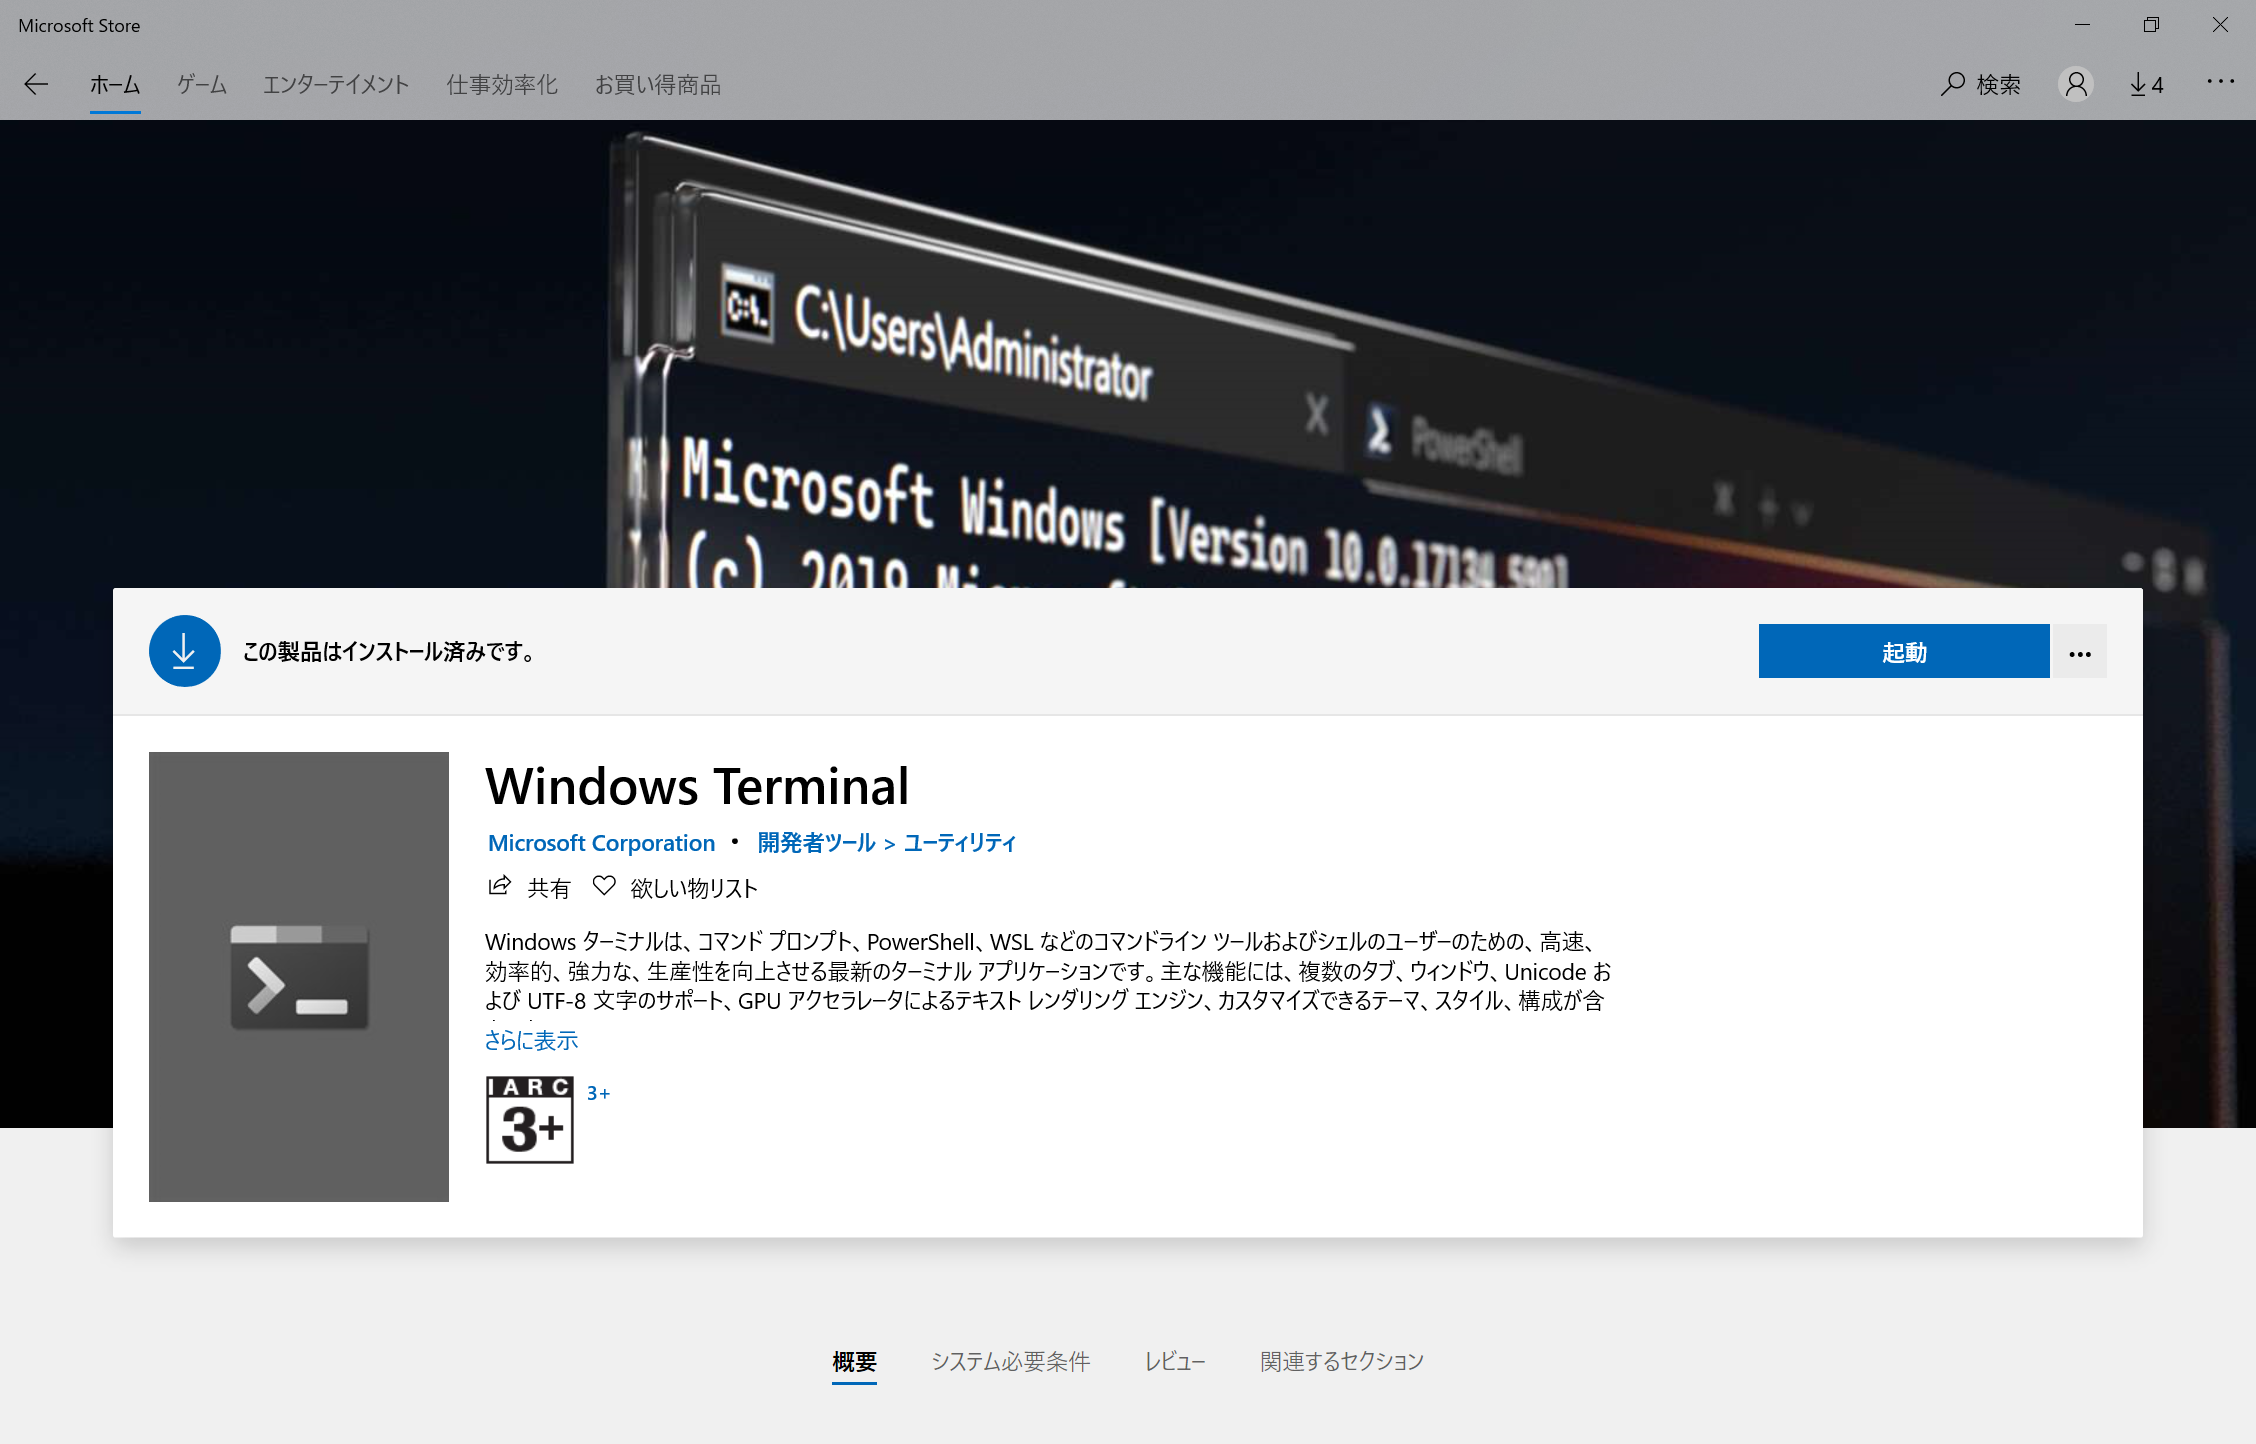
\includegraphics[scale=0.25]{./fig/install_terminal.png}
        \caption{Windows Terminalのインストール}
        \label{fig:install_terminal}
    \end{figure}
    \item PDFの場合
    \begin{figure}[H]
        \centering
        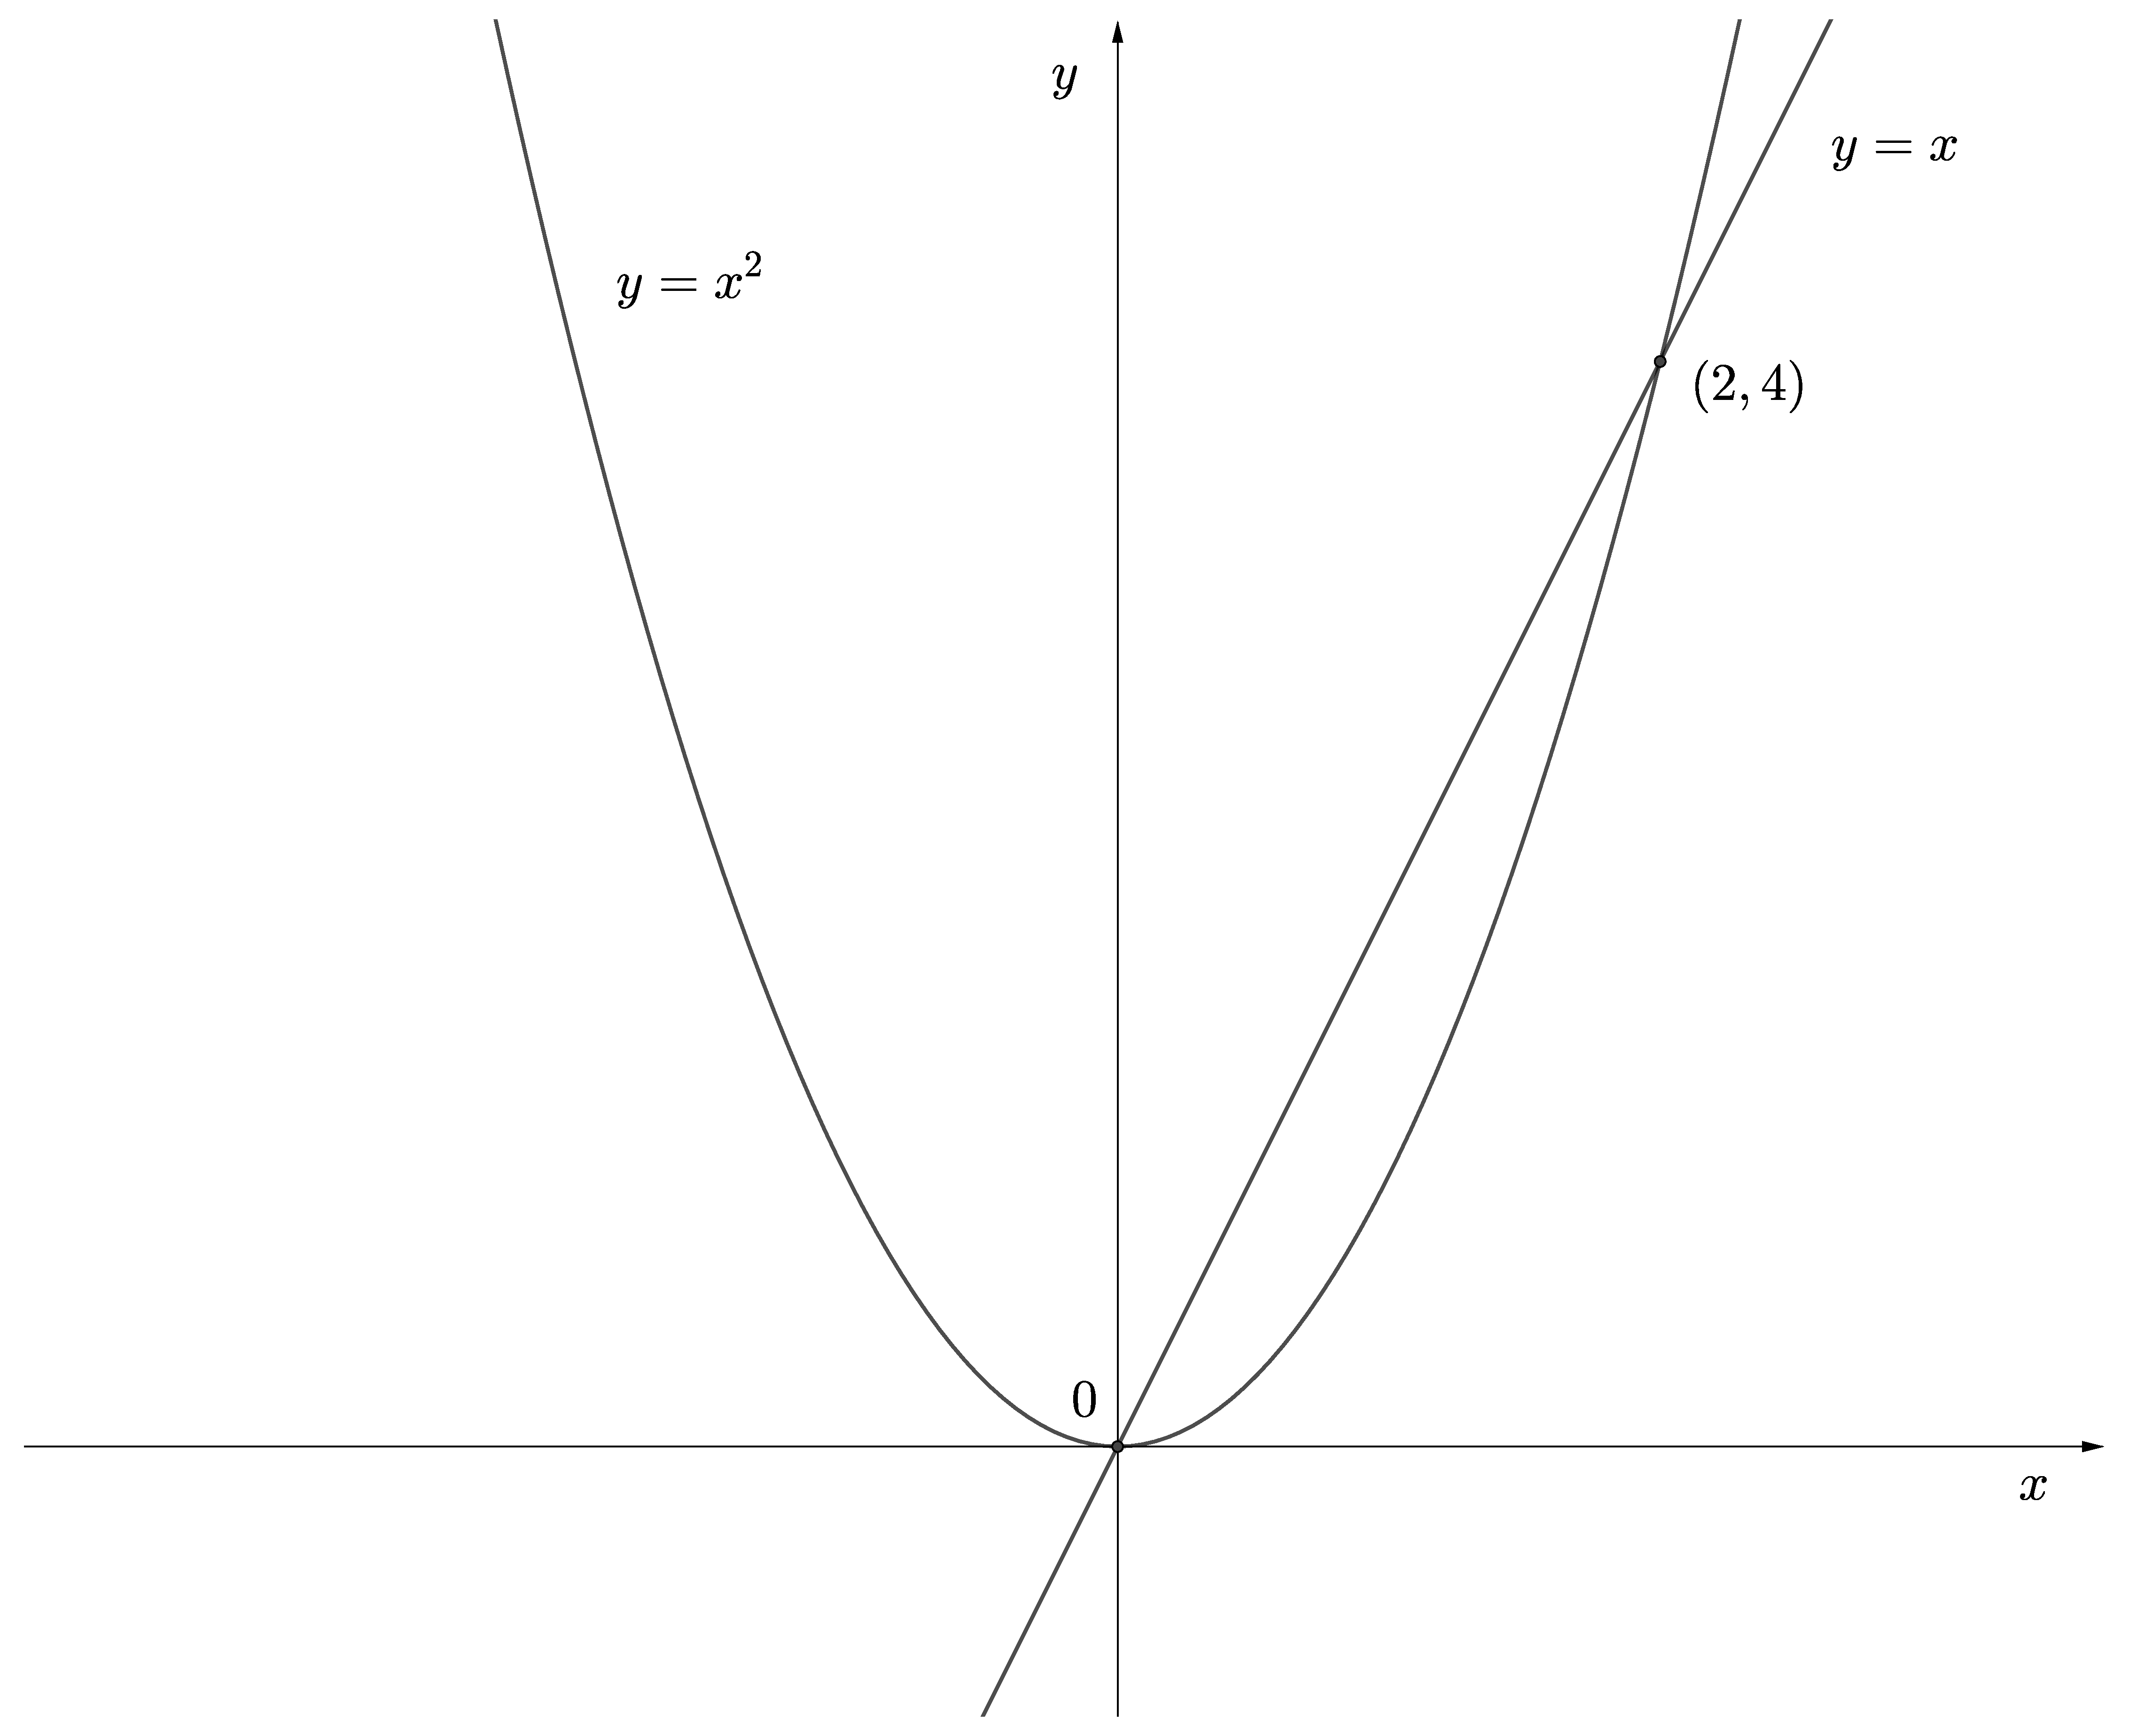
\includegraphics[width=0.5\textwidth]{./fig/graph.pdf}
        \caption{$y=x^2$と$y=x$のグラフ}
        \label{fig:graph1}
    \end{figure}
    \newpage
    \item PDFのページごとの場合
    \begin{figure}[H]
        \centering
        \fbox{
            \includegraphics[width=0.75\textwidth, page=3]{./fig/slide.pdf}
        }
    \end{figure}
    
    \noindent
    \textbf{タイトル}

    これでノート形式の資料も作れる.
\end{itemize}
\end{document}